%!TEX root = thesis.tex

\chapter{Introduction}
\label{chap:introduction}

\begin{chapquote}{Frederick Brooks, \textit{The Mythical Man-Month}, p.185}
``In spite of progress in restricting and simplifying the structures of software, they remain inherently unvisualizable, thus depriving the mind of some of its most powerful conceptual tools. This lack not only impedes the process of design within one mind, it severely hinders communication among minds.''
\end{chapquote}

Visualisations bridge the gap between understanding and enjoyment. In software, visualisations have for a long time attempted to provide a higher level of understanding but have rarely been effective in communicating the fundamental processes of software development. The Mythical Man-Month goes so far as to suggest that ``software is invisible and unvisualizable''\cite{Brooks1995} sparking debate as to the effectiveness of all software visualisations commonly used in the understanding and evaluation of software. 

Within the last two decades, the introduction of live coding has presented a unique application space for visualisations and the potential for effective communication through visualisation has been identified. These new developments could challenge the long-held belief that ``software is invisible and unvisualizable''.

The intention of software visualisations is to communicate software effectively. In recent years there has been a push to develop software visualisations further as the audience of software becomes more diverse, multidisciplinary teams within the industry become the standard and multimedia and the arts become more focussed on effective software development.
% link to live coding?

As the complexity of software increases, better methods are required for communicating software structure, software changes and, perhaps most importantly, communicating the process of developing software. Live coding is a means of combining the artistic goal of enjoyment and the educational aspects associated with programming with visualisations to effectively communicate software.

This thesis investigates the proposition that ``code visualisation improves observer understanding and enjoyment'' in the setting of a live arts practice. More specifically, this thesis investigates the question ``can the application of visualisation techniques to live coding enhance audience experience by increasing understanding and enjoyment?''. These questions were examined through a process of prototype development, user study evaluation and refinement.

% This project will examine the relationship between aesthetics and educational aspects of code visualisiatons applied to two fields - an industry based application and a new media art application. 
This thesis will explore the application of software visualisations to the process of live coding. A process of design iteration and evaluation was conducted in collaboration with a live coding musical artist to develop software visualisations. Three studies were administered, including one field study and two laboratory studies as a means to determine if understanding and enjoyment could be influenced by the introduction of visualisations to live coding.

% problem statement and tie in quote?

\section{Background}

Both visualisation and live coding have a long history of communicating intent. This section seeks to define visualisations, summarise the history of visualisation, how visualisation has begun to be used in the software industry, the contributions of live coding within this space and the potential for visualisations within live coding.

% Random stuff from early in the project:

% -code is often difficult to quickly understand
% -some observers may lack the experience to understand the software or the programming process

% Additionally, how we program does not achieve the goals we set out to achieve (from $https://www.youtube.com/watch?v=1f13TTu_X9k$, taken from presentation reimagining programming languages):
% -programming is unobservable (looking at the system through a keyhole)
% -programming is indirect (no direct feedback)
% -programming is incidentally complex (complexity not inherent in the problem that we need to solve)


% -how can we improve source code comprehension?
% -how can we aid understanding of the programming process?
% -better yet, how can we better communicate the programmers intention?

% -techniques such as modelling or code documentation aren’t dynamic or flexible
% -don’t allow for close to realtime understanding
% -an effective technique is the use of visualisations
% -it would be valuable to use visualisations as a means to communicate the programmer’s intention


\subsection{Software}
{\color{red} maybe remove this section as it is discussed in-depth in the next section...}

For most of its history, source code has been displayed as simple text. This is due to the expressiveness of the text format and despite its inefficiencies. It is only recently, due to ever increasing programming language complexity and increasing computational power, that code annotations and syntax highlighting have become more commonplace. Nevertheless, these visual enhancements rarely provide information beyond the basic grammar of the language they are intended to augment. The limitations of this approach are becoming ever more apparent as programming languages and interactive programming environments move towards the need for real-time comprehension and a need to understand the source code within the context of a running program.

% Discuss the software engineering approach here... applying software development techniques to an arts space. Identify stakeholders etc... Discuss how the project was undertaken regarding timelines and collaboration with the stakeholders...
% Push the software engy stuff here...
% eg. The purpose of software engineering is to bring together ideas from many fields into one - developing good software that is fit for purpose and fit for use. The systems engineering perspective of software engineering. However, one area where software engineering has had little influence and little influence has been taken from is the area of art.

Modern software is increasingly supporting the concept of the hotswapping of source code. Hotswapping source code is the process of modifying program source code at runtime to achieve desired behaviour without restarting the system. The ability to hotswap source code is becoming increasingly common within programming languages. Examples of this paradigm exist within Java including HotSwap, JRebel~\cite{ZeroTurnaround2014} and a variety of other custom modifications (e.g.~\cite{Thomas2011}). {\color{red} other languages...}

{\color{red} better link between paragraphs}

One area in width the paradigm of hotswapping source code is central is that of interactive programming, specifically live coding. Live coding is the process of programming in front of an audience for education or entertainment. It is a relatively new and developing field intending to further blur the lines between the worlds of art and programming. Live coding provides exposure of the programming process to a live audience, with the audience often having no background in programming.

Some of the most important and influential live coding environments over the last decade have included SuperCollider~\cite{McCartney}, ChucK~\cite{Wang2008} and Extempore~\cite{Sorensen}. These environments have a growing following as the field of live coding matures.

% -how has the increased dynamic nature of programming created difficulties in understanding.
% -how has the increased dynamic nature of programming languages made it more difficult to visualise? how has it made it easier?

\subsection{Visualisation}

\begin{figure}
\centering
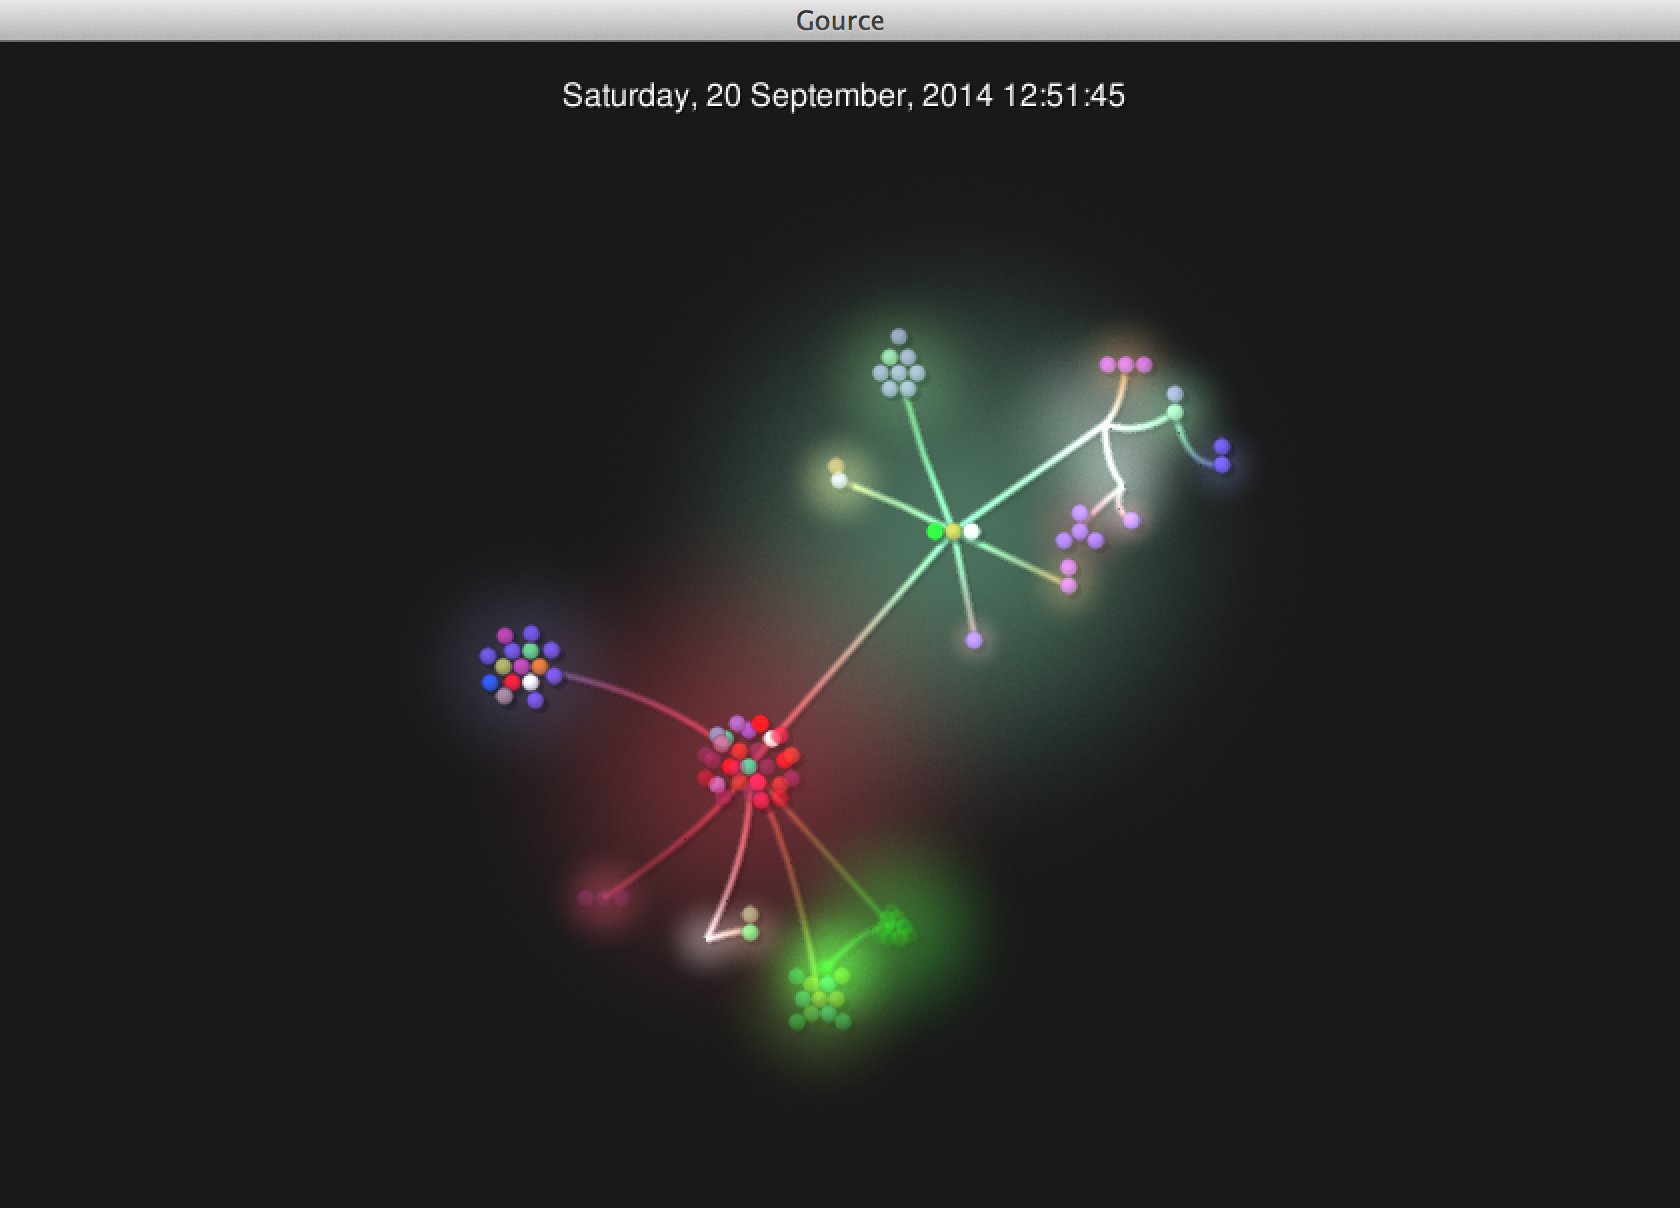
\includegraphics[width=1.0\textwidth]{../images/gource.png}
\caption{An example of Gource. This software visualisation shows each file in the software project as a node and orders the nodes according to the directory structure. Data is extracted from source code repositories.}
\label{fig:gource}
\end{figure}

Modern visualisation generally has two distinct definitions. The first definition involves representing data graphically while the other definition describes the process of forming mental visual images. {\color{red} Both processes can assist in the communication and understanding of information}

Since its inception, the visualisation of data has revolutionised how information is represented and understood. The earliest examples of summarising data using images occurred in William Playfair's \textit{The Commercial and Political Atlas}. Playfair developed a number of graphical representations of data that are very common today including the line chart, the bar chart and the pie chart.


% -software visualisations

% Discuss progress to computation of data on computers and effect on the direction of visualisation...

% Discuss information needs of the modern age...

Exisiting source code visualisations such as Gource~\cite{Caudwell2010} (see Figure~\ref{fig:gource}) and Code Swarm~\cite{Ogawa2012} show historic source code changes, based off source code respository data. Inline annotations~\cite{Swift2013} provide direct feedback directly useful to the programmer and technologies such Light Table~\cite{Kodowa2014} with an inline interactive terminal or \ac{REPL} have further identified the need to provide more visual information regarding active programs.

\section{Structure}

The structure of this thesis consists of Chapter~\ref{chap:literature-review} summarising the literature including the basis for and the direction of this thesis. Following this, Chapter~\ref{chap:exploratory-field-study} discusses the initial exploratory field study conducted to investigate existing perception and understanding of the live coding process. Chapter~\ref{chap:visualisation-design} discusses the first iteration of the visualisation prototype developed following the results of the exploratory field study. Chapter~\ref{chap:user-study} summarises the first user study conducted with the visualisation prototype. Chapter~\ref{chap:visualisation-refinement} discusses refinement of the visualisation prototype motivated by the results of the first user study. Chapter~\ref{chap:follow-up-user-study} discusses the follow-up user study conducted to analyse the refined visualisations. Chapter~\ref{chap:summary} summarises the results of the user studies, contributions, limitations and future work. Finally, Chapter~\ref{chap:conclusion} provides some final words to conclude the thesis.
% -will be using live coding as a platform and case study for this (will discuss later)\\
% -will develop and test code visualisations on audiences with audiences of varied levels of experience with programming, addressing code comprehension


